\documentclass[a4paper,11pt]{article} \usepackage[T1]{fontenc} \usepackage[utf8]{inputenc} \usepackage[francais]{babel}
\usepackage[top=2cm,left=2.5cm,right=2.5cm,bottom=2cm]{geometry} % Géométrie de la page, modifier selon le besoin
\usepackage{lmodern, textcomp, tikz, graphicx, amsmath, tikz-qtree, xcolor,rotating,epic,eepic}
\usepackage[colorlinks,linkcolor=black, urlcolor=blue]{hyperref}
\usepackage[babel=true,kerning=true]{microtype}
\usetikzlibrary{matrix, arrows, calc, shapes.geometric, shapes.misc, shapes.symbols, shapes.arrows, automata,
    through, positioning, scopes, decorations.shapes, decorations.text, decorations.pathmorphing, shadows}

\begin{document}
\pagenumbering{gobble}  % Pas de numérotation
\begin{titlepage}

\includegraphics[scale=0.45]{Public/logo_phelma.pdf}\hfill
\includegraphics[scale=0.55]{Public/logo_robotronik.png}
\begin{center}
    \vspace*{2cm}
    \rule{\linewidth}{0.5mm}\\[0.4cm]
    {\huge\bfseries Demande de reconnaissance pour investissement dans des activités associatives\\
    [0.4cm]}\rule{\linewidth}{0.5mm}\\[1.0cm]
    \large{\textsc{Robin Moussu}}
    \begin{flushright} \large
        2\ieme Année \\
        Filière \textsc{SLE} \\
        Responsable informatique et électronique \textsc{Club Robotronik}\\
    \end{flushright}
    \vfill

    \large{\today}
\end{center}
\end{titlepage}
    \tableofcontents        % Table des matières avec liens, générée automatiquement.
\newpage
\pagenumbering{arabic}  % Numérotation de retour !
\part{Informations sur l'Association}
    L'Association Robotronik (appelée aussi le Club Robotronik) a été créé en 2008, suite à la fusion de PG Robotik
    et du Club Électronique.\\

    Le Club a pour vocation tout d'abord de faire découvrir aux étudiants de Phelma les vastes domaines de la Robotique.
    Il organise et participe à quelques événements en-dehors du Club, comme la Fête de la Science qui s'est justement déroulée ces vendredi et samedi.\\

    Il a donc aussi pour but d'être présent aux différentes manifestations telles que la Fête de la Science,
    pour promouvoir la Robotique au public.\\

    L'objectif du Club chaque année est de participer à la Coupe de France de Robotique, qui rassemble près de
    200 équipes de jeunes à La Ferté-Bernard, dans une ambiance conviviale autour de la Coupe.\\

    Le club regroupe aujourd'hui 7 Deuxièmes Années, ainsi qu'une douzaine de Premières Année. Il permet, de façon très exceptionnelle, à des élèves extérieurs à participer au travail du club.

\part{Le rôle que j'exerce dans le Club}

En tant que responsable informatique, mon rôle est de faire en sorte que chacun des membres ait les connaissances lui permettant de participer efficacement au projet. Pour cela je me suis fixé le rôle de donner des cours d'informatique aux différents membres du club, notamment ceux de 1\ieres{} année. En effet, nous utilisons de nombreux logiciels qu'ils ne connaissent pour la plupart pas encore lors de leur arrivée à Phelma.

Pour cela, j'organise depuis le début d'année des cours dont le but est de maitriser les outils utilisés au club. Ces outils sont notamment git et doxygen, mais je compte également donner aux membres des conseils pour qu'ils aient de bonne méthodes de programmations. Enfin je leur transmettrais des notions spécifiques aux micro-contrôleurs(interruptions, PWM, registres…).

La connaissance de ces outils peut-être réutilisé plus tard dans le cadre de notre formation à Phelma ou en tant qu'ingénieur. Leur apprentissage est donc très bénéfique. C'est une des raisons qui m'ont poussés à choisir des outils les plus standards possible.\\

    De plus en tant que responsable tant informatique qu'électronique, j'ai pour charge de valider les productions du club dans ces domaines. Cette validation a été mise en place afin de garantir la qualité des productions effectués aux clubs. De plus cela permet d'avoir des productions dont le style est uniforme. Florence André à le même rôle pour la partie mécanique.

    Durant mon cursus, j'ai déjà participé à  trois coupes de robotiques (deux fois la coupe de France, et une fois la coupe inter-IUT), ce qui m'a permis de gagner de l'expérience dans le domaine de la robotique. J'ai également beaucoup programmé sur mon temps libre. Ayant fait un UIT GEII, j'ai acquis de bonnes bases en électronique. Le fait d'être responsable électronique et informatique me permet de transmettre au mieux cette expérience, et d'en faire profiter les autres membres.\\

    En tant que membre actif, j'ai décidé d'améliorer la communication interne du club, afin de faciliter la transmission de connaissance d'une année à l'autre. J'ai par exemple participé à la mise en place d'un wiki cet été.

    Je suis enfin impliqué dans les différents projets du club, tout spécialement la coupe de France qui est pour moi un évènement très important.

    \begin{figure}[h] \begin{center} 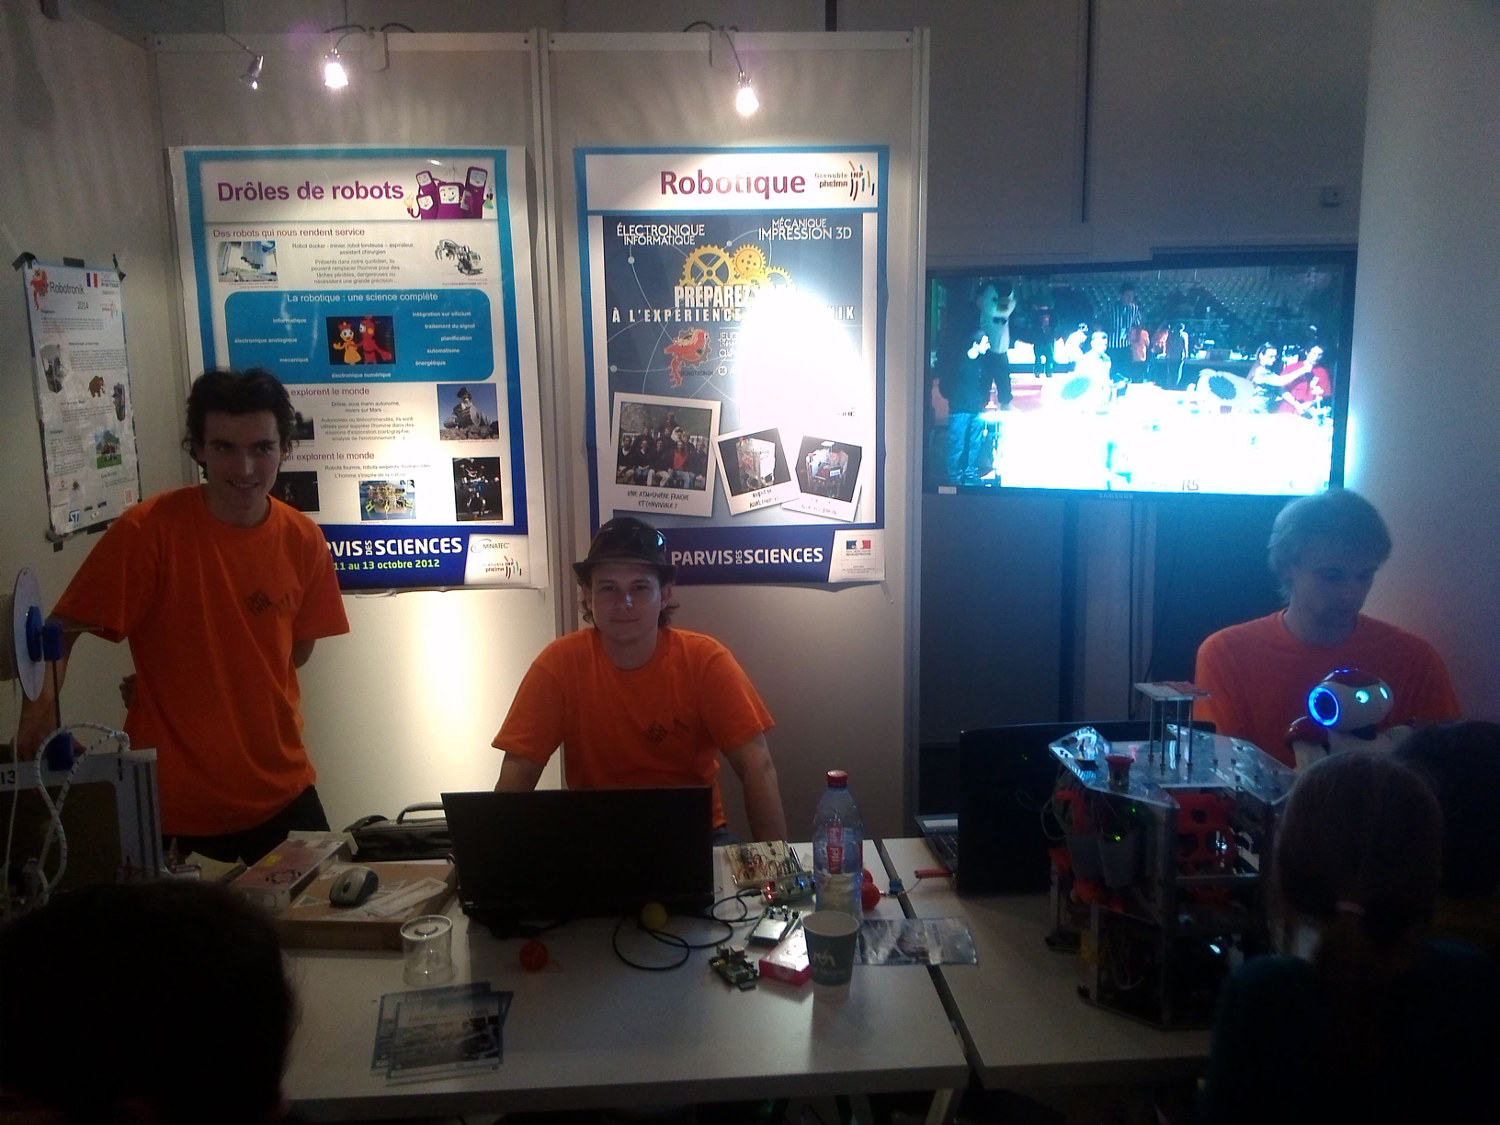
\includegraphics[width=250px]{Images/FeteDeLaScience}
        \caption{Le Stand Robotronik à la Fête de la Science, samedi 11 octobre 2014} \end{center} \end{figure}

\part{Mes objectifs et ceux du Club}

Mes objectifs en tant que membre du club sont évidement que les projets du Club réussissent. Le plus important de ces projets est évidement la coupe de France de Robotique à la Ferté Bernard en Mai 2015.\\

En tant que responsable informatique, mon rôle est de garantir que le code qui va être développé cette année soit fonctionnel, mais également qu'il soit maintenable et documenté, afin de pouvoir le réutiliser l'an prochain, malgré le renouvellement des membres.

De plus, une partie du code des années précédentes n'est pas documenté. Je vais donc faire en sorte que cela soit corrigé, afin de produire un travail de meilleure qualité.\\

En tant que responsable électronique, mon but est de garantir que les cartes produites soient fonctionnelles, avec un minimum de défauts possibles. Durant mes 2 années en passé IUT, ainsi que l'an dernier à Phelma, j'ai réalisé de nombreuses cartes, et ait acquis de l'expérience que je souhaite transmettre au club. De nombreuses cartes vont devoir être réalisé cette année, entre autre dû à des changements de technologie (batteries Li-Po et micro-contrôleurs STM32 essentiellement).\\

Pour résumer, j'estime que mon rôle dans le club est essentiellement de transmettre mes connaissances et d'être le garant de la qualité des projets du club dans les domaines qui me concerne.

Je ne suis bien sur pas le seul dans le club à avoir ce rôle. Ojeme Ikhalo me seconde pour ce qui est modélisation 3D, car il est plus compétant que moi. Enfin Florence André s'occupe de superviser les productions mécaniques du club.

\part{L'apport d'expérience pour mon futur métier d'ingénieur}

En tant que responsable dans le club, je vais devoir encadrer d'autres personnes. J'aurai donc un rôle de manager. Cela me sera particulièrement utile en tant qu'ingénieur, car l'encadrement de personnel, et le travail en équipe feront partie intégrante de mon travail.

J'aurai également un rôle de formateur. Avoir des compétences pédagogiques est toujours utile dans le cadre d'un travail en équipe, car elles facilitent la transmission de connaissances, et demande des facilitées d'adaptation.\\

En tant que membre du club participant à la coupe de France, je vais devoir mener à bien un projet. Ce projet sera une production collective, et nécessite que le club soit efficace. Par conséquent, être membre dans le club Robotronik est très formateur pour le travail en équipe. Enfin je vais devoir travailler ma gestion du stress durant cet évènement.

\part{Organisation du Club sur l'année}
Bien sûr, l'échéance principale du Club est la Coupe de France de Robotique, mi-Mai.

Mais nous avons décidé comme échéance idéale la pré-coupe de Lyon qui a lieu en mars. Cela nous donnera le temps d'améliorer et de paramétrer nos robots en fonction des résultats que nous aurons obtenus.\\
\begin{figure}[h]
    \begin{center}
        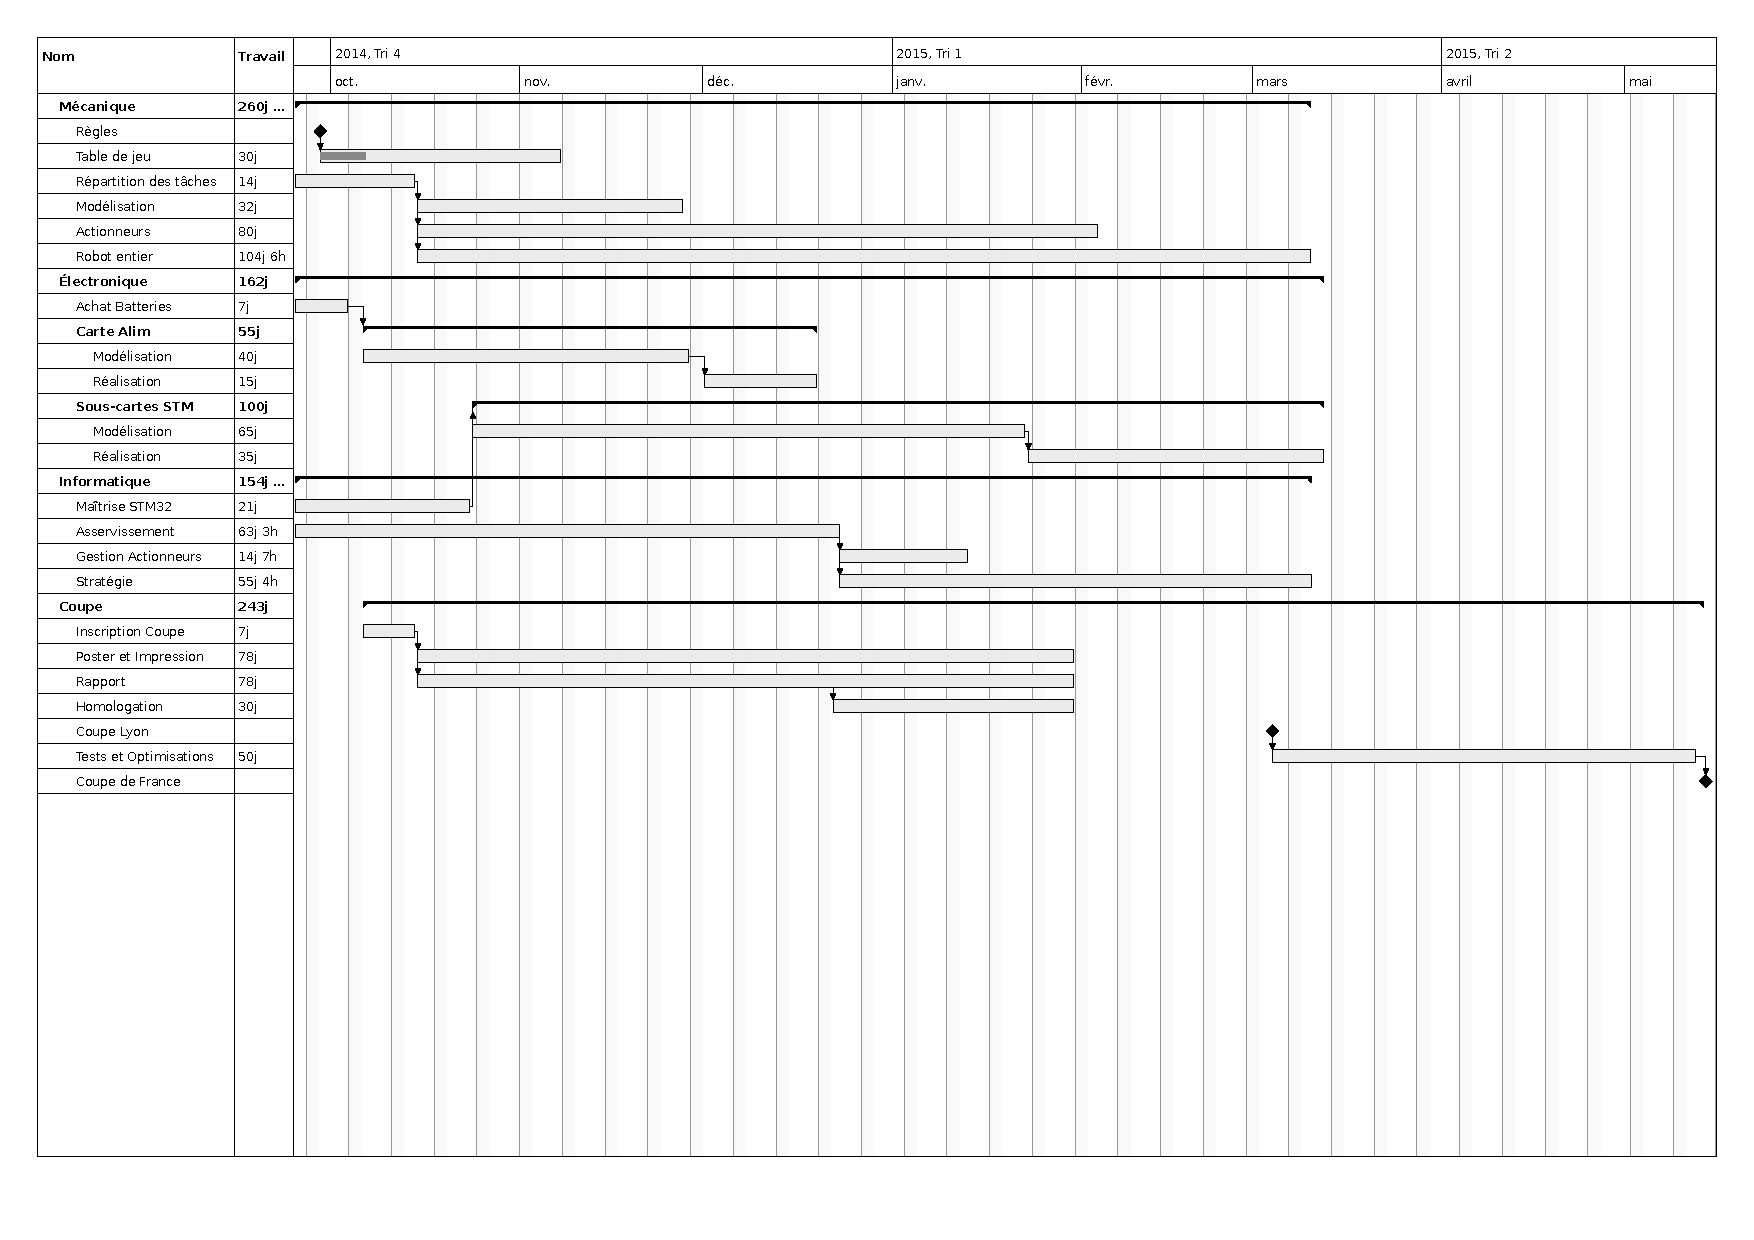
\includegraphics[trim=27px 215px 17px 33px,clip=true , width=\textwidth]{Public/GanttRobo.pdf}
        \caption{Gantt du Club Robotronik}
    \end{center}
\end{figure}

L'échéancier se divise naturellement en trois catégories (en ce qui concerne la partie technique) que sont les composantes du club : mécanique, électronique et informatique.

Les trois parties ne sont bien entendu pas indépendantes, mais nous pouvons débuter chacune séparément, afin de préparer certains aspects de l'informatique qui ne dépend pas du robot -- mais qui doivent être refait avec les changements techniques décidés -- ou les cartes de protection des batteries côté Électronique.\\

La modélisation de la mécanique pose les bases nécessaires au dimensionnement de l'électronique, mais bien sûr nous serons confrontés à des problèmes de réalisation. C'est pourquoi nous devons avancer au plus vite sur la mécanique pour déterminer les modifications à effectuer sur l'électronique, et pour permettre à l'informatique d'être finalisée, évaluée et calibrée.\\

Mon implication temporelle dans le cadre du club robotronik est de 4h30 par semaine plus en moyenne deux heures pour préparer les séances (notamment les cours de début d'année), ce qui fait un total de 6h30. De plus, nous aurons à passer plus de temps en fin d'année pour la réalisation des robots participant à la coupe.

J'estime donc à 250 heures le temps que je destine au Club durant l'année, sans compter la Coupe qui se déroule sur cinq jours mi-Mai.


\part{Périodes et contenus (livrables) – Présentation du déroulement de l'activité (et point de suivi) }

Le principal projet du club est bien sûr la Coupe de France, mi-Mai. Mais comme je l'ai dit plus haut, nous devons être prêt pour la pré-coupe de Lyon en mars. Cela nous permettra de visualiser les différents problèmes et améliorations sur nos robots afin d'y remédier avant la Coupe.\\

De plus, plusieurs évènements se déroulent tout au long de l'année.

Notamment ce vendredi 10 octobre a été finalisé le char de Phelma pour les Ol'INPiades, pour lequel nous avons réalisés des yeux lumineux. Samedi a eu lieu la Fête de la Science, pour laquelle nous avons eu à préparer des animations avec le Nao, une imprimante 3D et notre robot qui a participé à la Coupe l'an dernier.

Nous devons également finir la table de jeu début novembre, et concevoir  des cartes de gestion des nouvelles batteries LiPo qui devront être "livrables" mi-décembre.\\

\newpage
\begin{center}
\pagenumbering{roman}
\addcontentsline{toc}{part}{Annexes}
\setcounter{page}{0}
\vspace*{10cm}
{\huge\bfseries Annexes\\
[0.4cm]}\rule{\linewidth}{0.5mm}
\end{center}

\newpage
\section{Organigramme du Club Robotronik}

\vspace*{3cm}
\begin{center}
\begin{tikzpicture}
\tikzstyle{bureau}=[rectangle, minimum height=1.8em,fill=yellow!30,text=black]
\tikzstyle{respo}=[rectangle, minimum height=1.8em,fill=blue!20,text=black]
    \node[bureau] (Prez) at (0,0) {Félix Piédallu, Président};
    \node[bureau] (Trez) at (-5,-1) {Ojeme Ikhalo, Trésorier};
    \node[bureau] (Secr) at (+5,-1) {Florence André, Secrétaire};
    \node[respo] (Chef) at (+0,-2.3) {Johan Lafon, Chef de Projet};
    \node[respo] (Elec) at (-5,-4) {Robin Moussu, Respo Électronique};
    \node[respo] (Info) at (+0,-5) {Robin Moussu, Respo Informatique};
    \node[respo] (Meca) at (+5,-4) {Florence André, Respo Mécanique};
    
    
\tikzstyle{ens}=[<->,dotted,very thick,>=latex]
\tikzstyle{sup}=[<->,dotted,very thick,>=latex]
    \draw[ens] (Chef) -- (Meca);
    \draw[ens] (Chef) -- (Info);
    \draw[ens] (Chef) -- (Elec);
    
    \draw[sup] (Trez) -- (Prez);
    \draw[sup] (Secr) -- (Prez);
    
    \draw[sup] (Prez) -- (Chef);
    \draw[sup] (Trez) -- (Chef);
    \draw[sup] (Secr) -- (Chef);
\end{tikzpicture}
\end{center}
\vspace*{7cm}
\begin{figure}[h]
    \begin{flushright}
        Le Président, Félix Piédallu, le 9 Octobre 2014,\\
        
\includegraphics[width=100px]{Public/SignaturePresident}
    \end{flushright}
\end{figure}

\end{document}
